%!TEX root = ../master.tex
\chapter{Discussion}\label{ch:discussion}
This chapter contains discussion of the entire project

\section{Sources of error}
Since the final test was conducted on 14 Medialogy students and one Art \& technology student, is it difficult to say whether the product would be just as usable for a random museums visitor or any other user. To investigate if the product would be understood amongst users with no knowledge of audio processing, the optimal solution would be testing the product in a context. The context in this case could be at an art museum, where the product would be tested on random visitors of all age groups.

From the test facilitators and the secretaries perspective some of the participants answers of whether they were able to hear the difference between the three filters effects were not clear enough. It was indicated the participants had a doubt if the noise came from the effect applied or the image itself, since the audiolosation of the image could been mistaken for effects. This problem could potentially have been tackled by having an additional test for just the effects by applying them on familiar sounds such as a continuous bell ringing or bird chirping. 

During the testing, when asked if the participants had any further comments to the prototype, a few participants mentioned they could hear the effects better on ‘Trolden og Fuglene’ compared to the ‘Mona Lisa’. This is not to be confused with the results on Tables \ref{tab:comb}, \ref{tab:bandpass}, \ref{tab:highshelf}, whether there is a difference between ‘MAX’ and ‘MIN’ of the three filters on both paintings, but it comes down to the whether the image itself and the implementation of the filters has anything to do with how intense the effect itself !comes of as!. Since only a few participants had that opinion, there was not enough data to support that claim for us to be able to conclude anything from it. It would be useful to actively examine this with interview questions that relate to this.

\section{Wider Context}
During this project, two of the members of the project group spend a day visiting the art museum Kunsten in Aalborg. The goal was to find out how the artefact could be used in context at the museum. With the non finished product in mind, the group members studied the different art exhibitions and tried to imagine the product in context with the art.

During the visit, three exhibitions, as can be seen on Figures \ref{Fig:Kblod}, \ref{Fig:aftryk} and \ref{Fig:chalk}, were considered the main inspiration for the context of use. These images were used to create sketches of the project artefact as a set up in an art museum as seen in Figure \ref{Fig:productsetupsketch}.

\begin{figure}[!h]
\centering
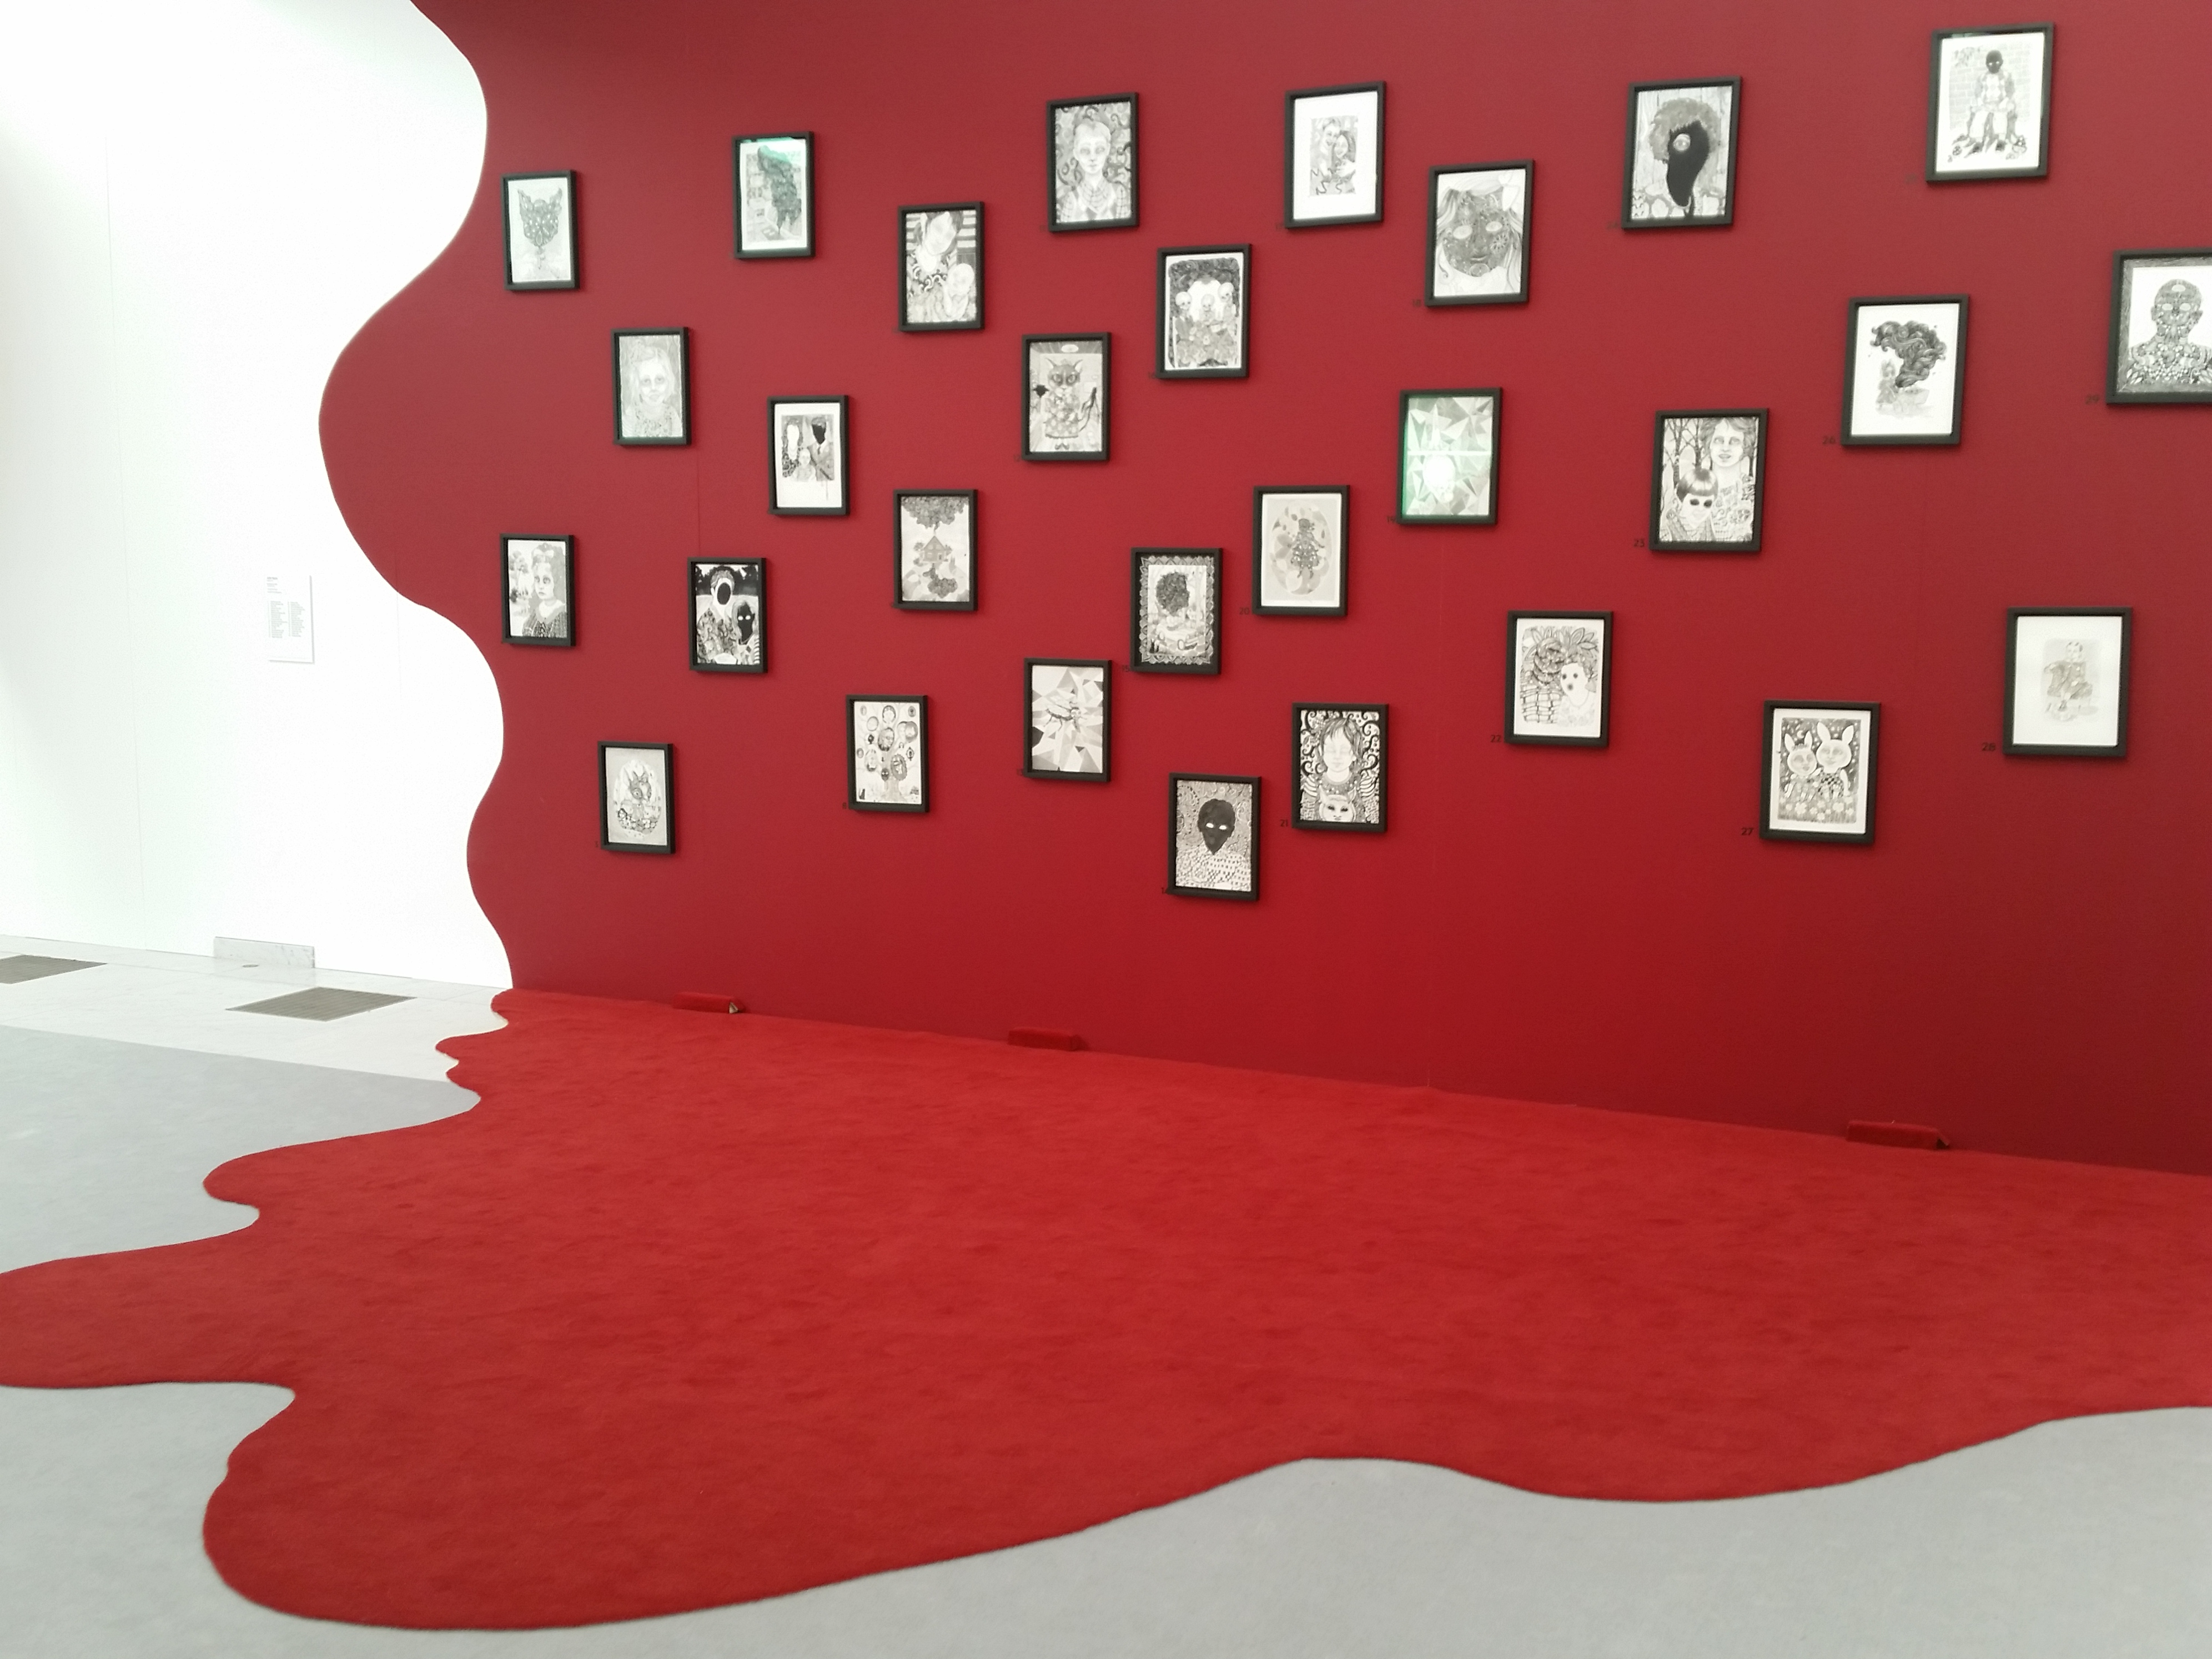
\includegraphics[width=1\textwidth]{Kblod}
\caption{\label{Fig:Kblod} Picture taken from Kunsten.}
\end{figure}
The art piece on Figure \ref{Fig:Kblod} creates a connection between the wall and floor with the red carpet. Inspiration was taken from this piece because the red colour of the floor and wall indicates that the two are connected. The group saw a need to establish an understanding of connectivity between the paint that is being audiolised and the artefact.

\begin{figure}[!h]
\centering
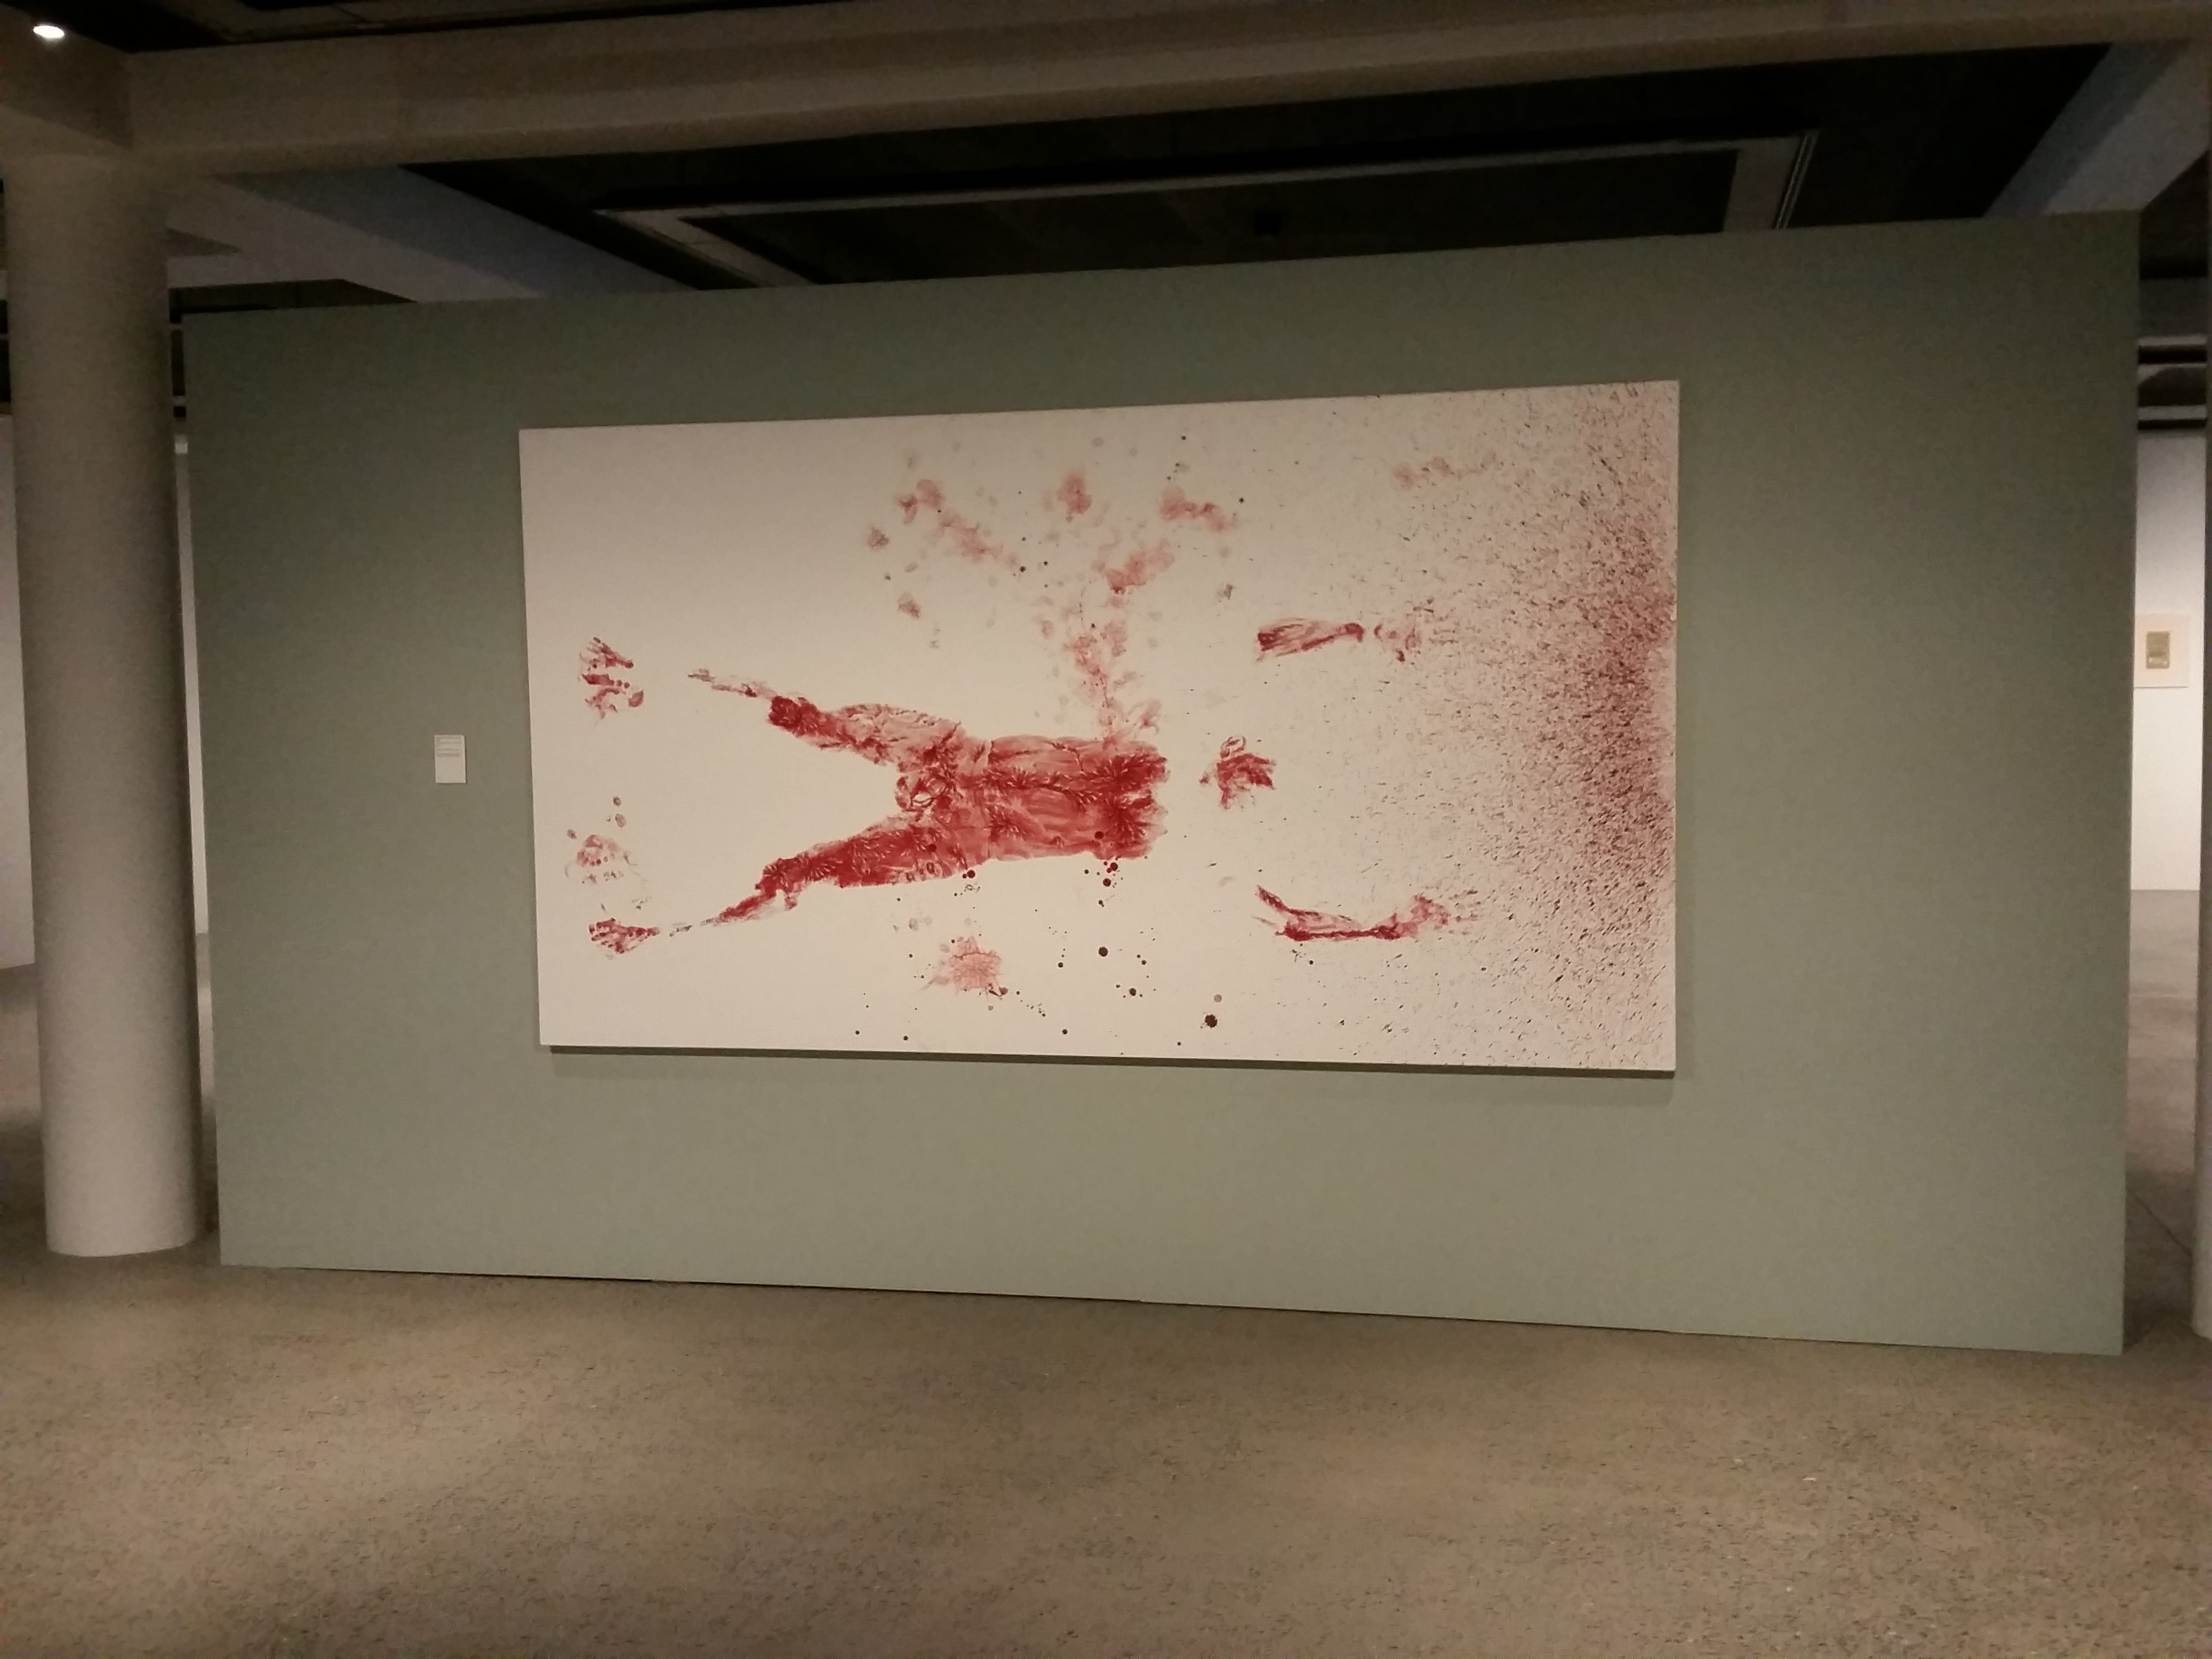
\includegraphics[width=1\textwidth]{aftryk}
\caption{\label{Fig:aftryk} Picture taken from Kunsten.}
\end{figure}

The art piece in Figure \ref{Fig:aftryk} has its own isolated wall with no sharing of space with other art pieces. Since the main project deals with audio, it was decided that it would be optimal for the product to be isolated from other art exhibitions to not disturb the visitors with loud noises.

\begin{figure}[!h]
\centering
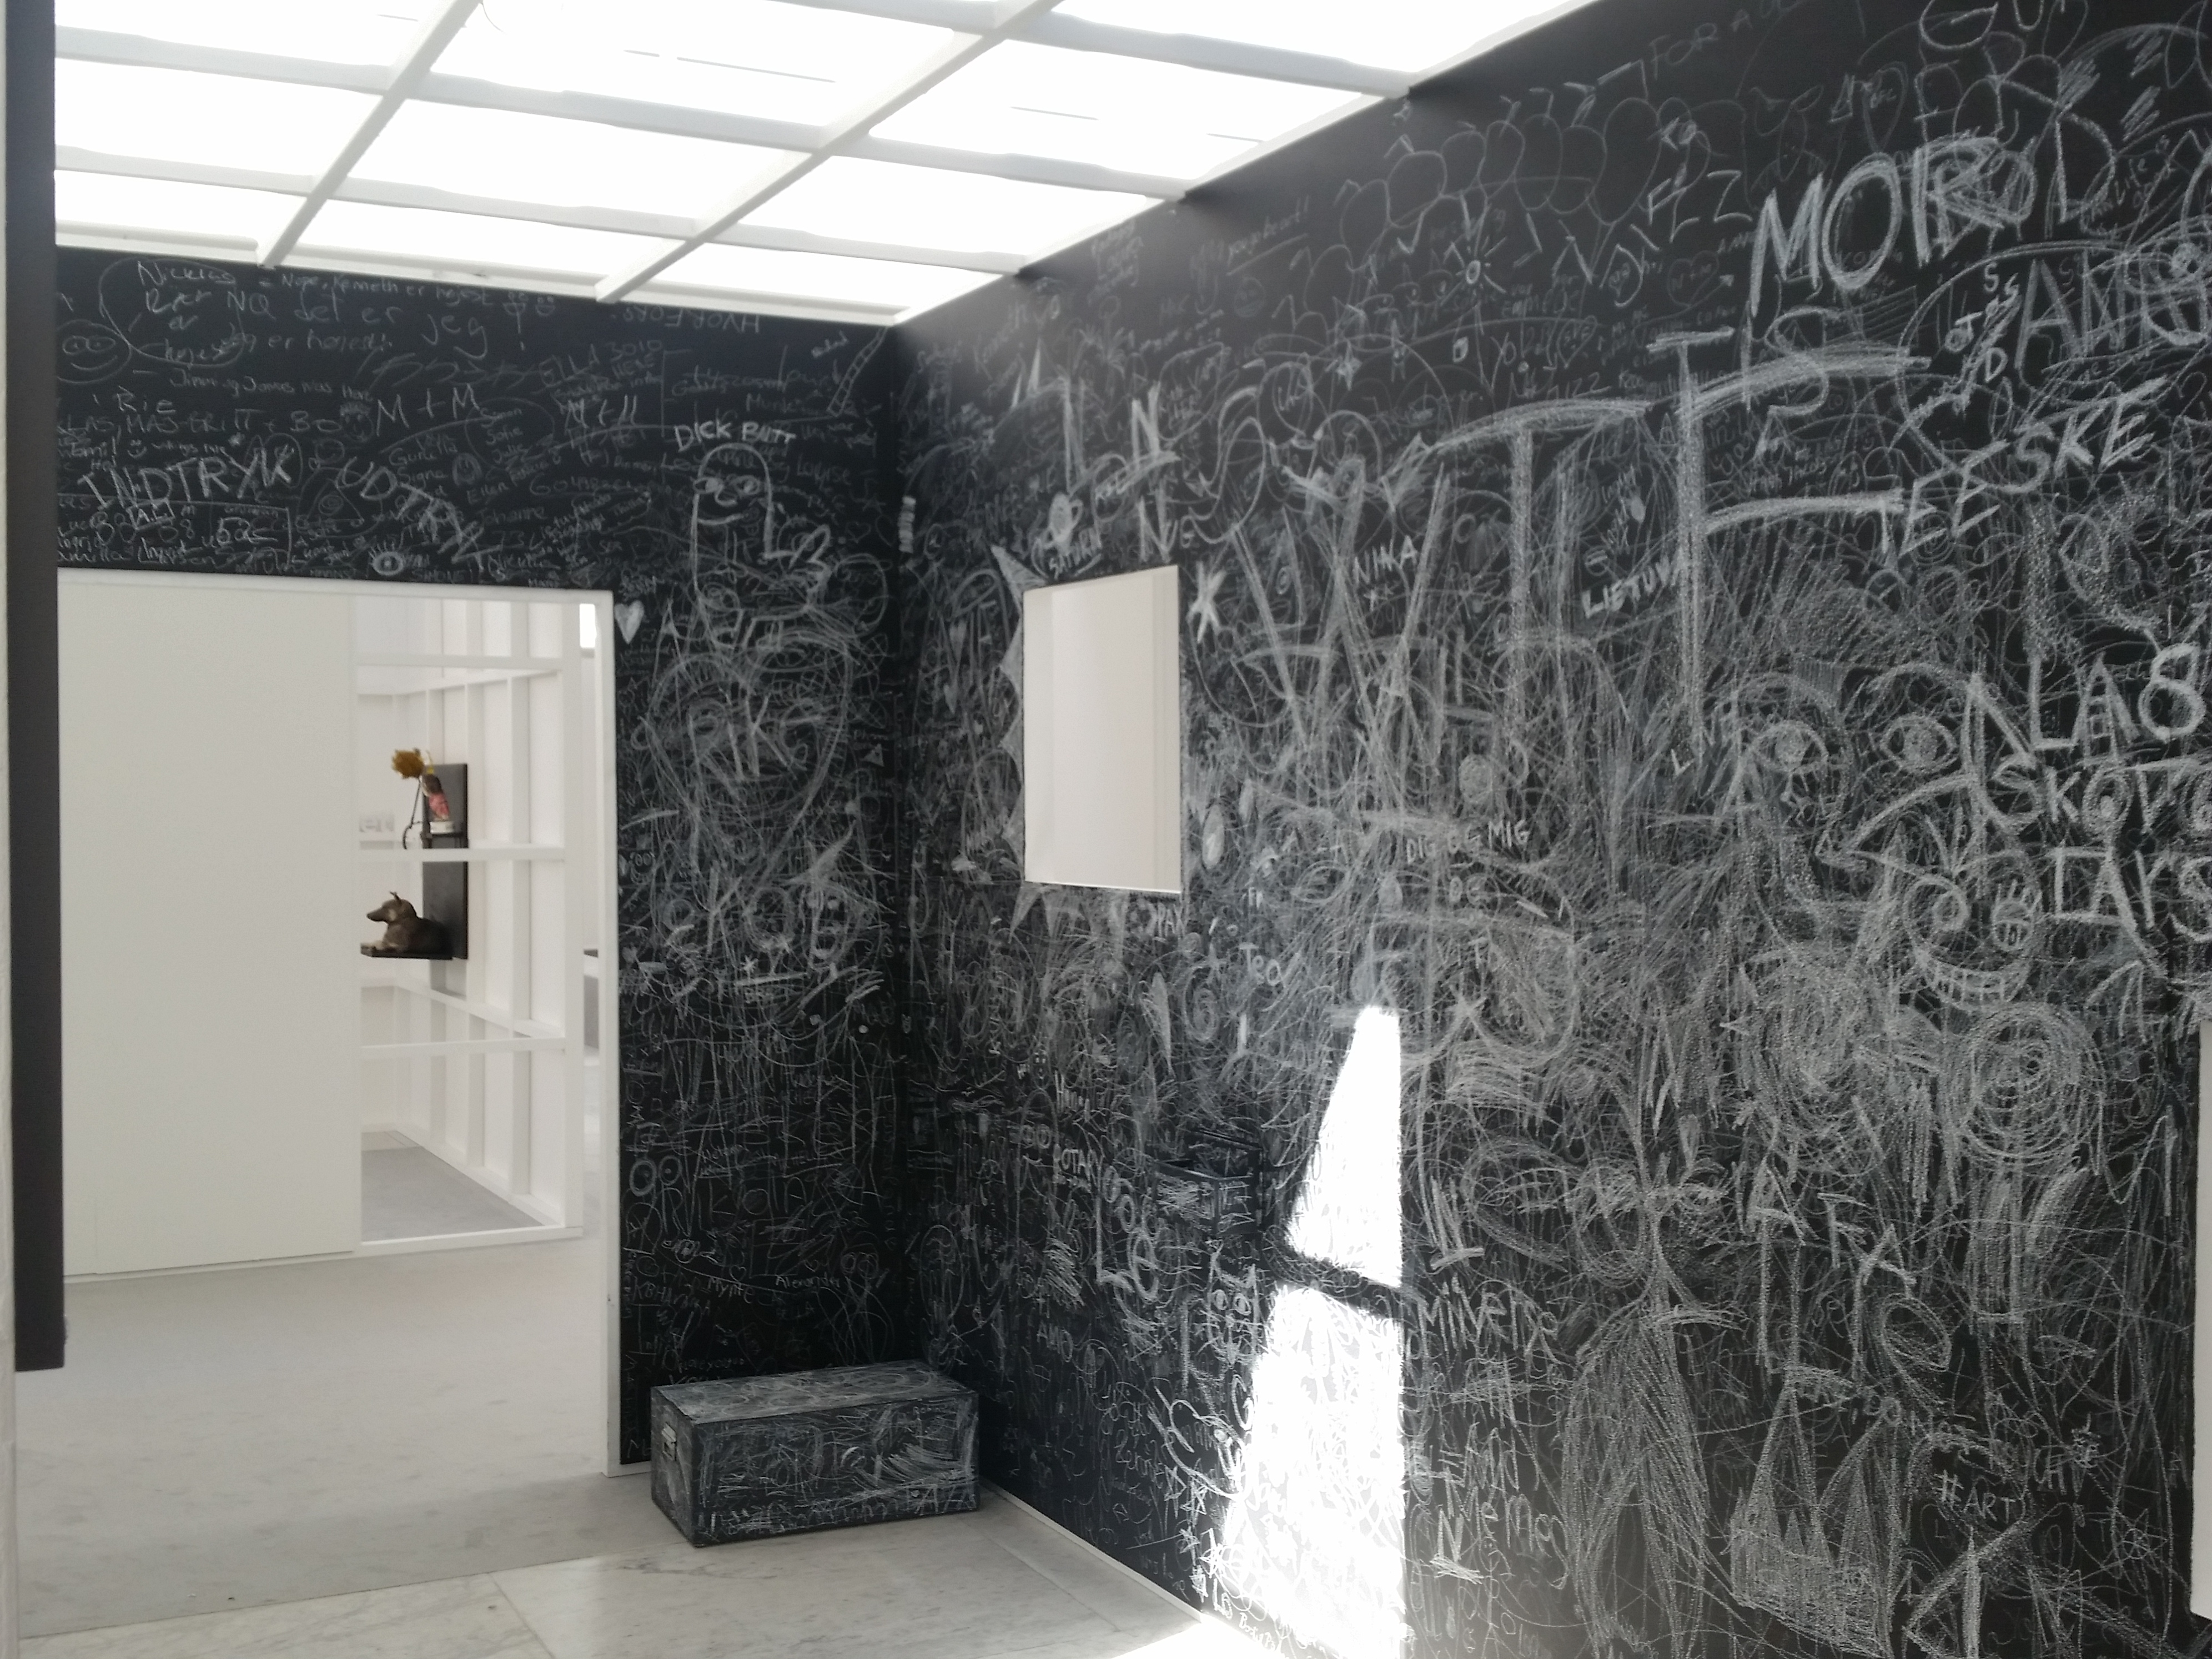
\includegraphics[width=1\textwidth]{chalk}
\caption{\label{Fig:chalk} Picture taken from Kunsten.}
\end{figure}

This interactive art piece as seen on Figure \ref{chalk} is in a closed space and it encourages the visitors to interact with it by drawing on the walls with white chalk. Since the main project is about making the people interact with the product, the group took inspiration from this art piece by looking at its simplistic method of conveying the intended interaction.

The visit at Kunsten resulted in a sketch of how the product could potentially be used in an art museum context. The sketch seen on Figure \ref{Fig:productsetupsketch} utilises the color relationship between the artefact and the painting that is being audiolised as seen in Figure \ref{Fig:Kblod}, the need for isolation from Figure \ref{Fig:aftryk} and lastly a simplistic, interactive design from \ref{Fig:chalk.}

\begin{figure}[!h]
\centering
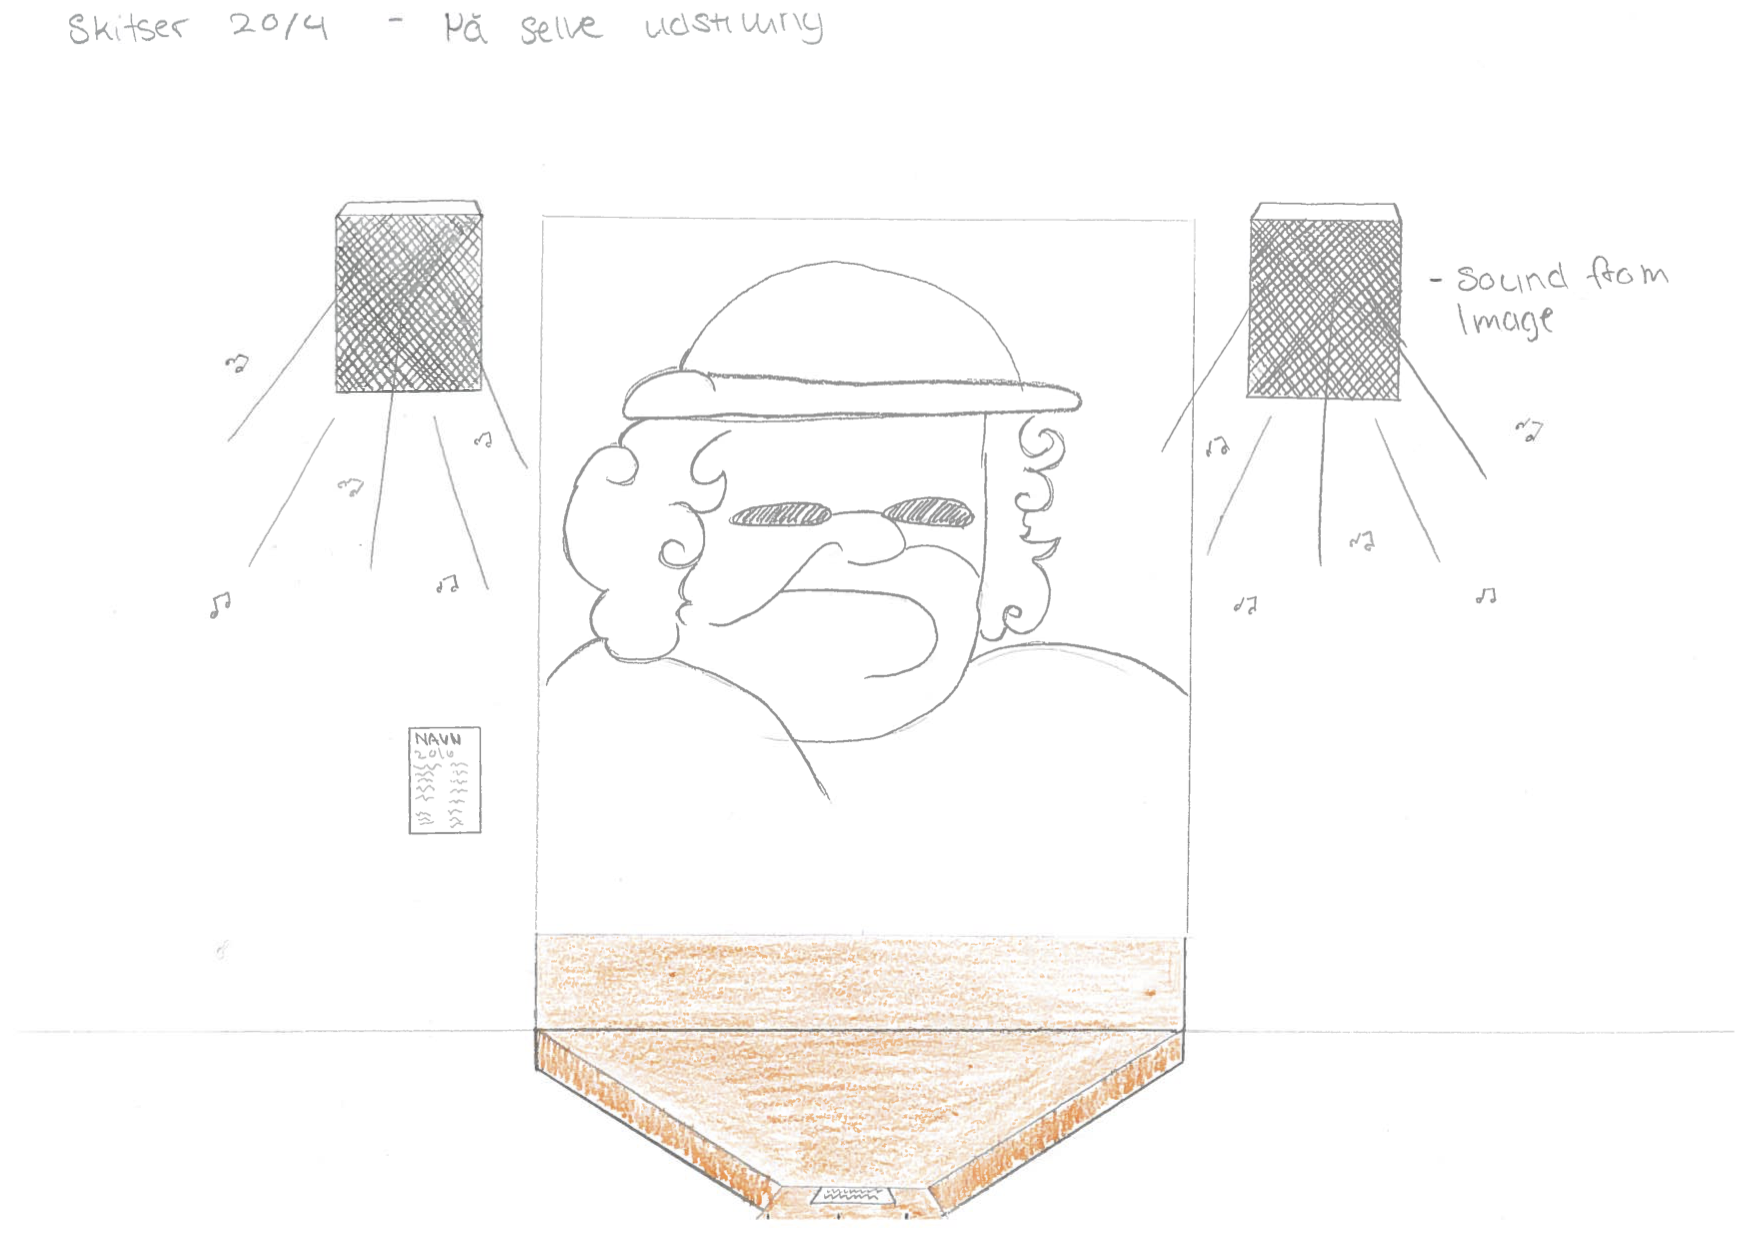
\includegraphics[width=1\textwidth]{productsetupsketch}
\caption{\label{Fig:productsetupsketch} Sketch of an idea, on how to set up the product at an art museum.}
\end{figure}

\section{Further Implementation}
For further implementation, If the filters had been applied differently so instead of a filter on each colour, it would be the total colour value that had the three filters applied. It could give a more clear effect, because it would affect one sound, instead of one out of three sounds.
The result might have been different if other filters were used, likewise if filter such as reverb, wah wah, or flanger were applied it might have given different results, due to the user being able to more clearly hear the difference between them. If the image was also changed, it would affect the RGB values, which would produce a different sound. This could have an effect on if the user could hear a significant difference between the pictures.

The results of the testing seen in Table \ref{tab:twoimagedifference} shows that the picture used have an effect on whether a filter can be heard, due to each filter being connected to a colour channel. If a picture with no green is used, one of the filters would be useless, due to it never getting any values. This would mean that if different pictures were used, with an equal amount of RGB, it could help the users ability to clearly hear the filters being applied.

It would be possible to alter the function of the project, such that the user would have the possibility to decide where in the picture the program should be looking, as this would allow the user further freedom over the creation of sound, made by the product. But if it was not implemented correctly, it would add to the confusion of the user, due to the amount of extra components on the interface. It could be done using an array of various components, such as a controller, slide potentiometers, or rotary encoders.

Instead of choosing where in the picture to look, the user should be able to create the picture in utilisation by the software. This could allow the user to differentiate themselves from each other, and create unique and interesting sounds, increasing its potential as a creative tool for artists as well as non artists. This could also make it an entertaining product to have at festivals, events, or at a museum.

An alternative version of the product, could be instead of a picture, it worked with a video feed, allowing it to render and manipulate the information given in real-time. This allows the user to translate his surrounding to sounds, giving a new perspective on the world. If this could be implemented onto a hand-held device, the user would be able to use things such as mobile phones or tablets. Which would allow the user to translate various areas without the need for a big machinery.
The user could also have the possibility to upload their own pictures, videos, or even add their own sounds which are played when translating.

During a discussion, it was suggested that the product could be used in other context like at a music or art festival. The idea was, that if the product should be should be presented at a festival, it had to have some changes to be suitable for the location. An idea was to make the product portable by putting it on wheels for easier transportation and elevate the electronic part of the product to prevent it from taking water and dirt in. In the figure \ref{fig:vidreudvikling} iswe see a sketch on how the portable version could look like.

\begin{figure}[!h]
\centering
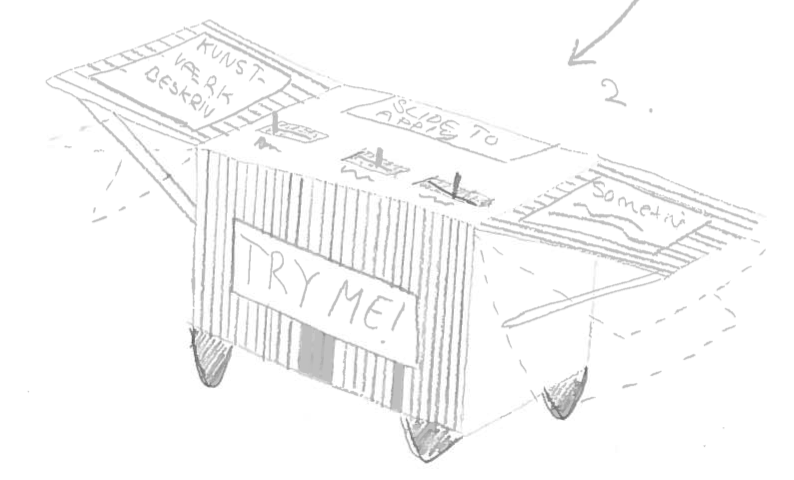
\includegraphics[width=0.5\textwidth]{vidreudvikling}
\caption{\label{fig:vidreudvikling} Sketch of how the portable version could look like.}
\end{figure}

During the final test, one of the test participants was unsure of the connection between the artefact and the paintings shown during the test, he needed to be explained that the sound was made by the painting, as this was not clear. Ideas were made to visualise the sound on the actual painting like shown in \ref{fig:Visualiseringaflyd} \todo{måske skald er tilføjes lidt mere, men ced ikke helt hvad} But if it is not clear to the user, it might just give the impression of an equaliser on top of a picture, confusing the user about what is producing the sound, but it would make it more clear whether or not an effect is being applied to it. 

\begin{figure}[!h]
\centering
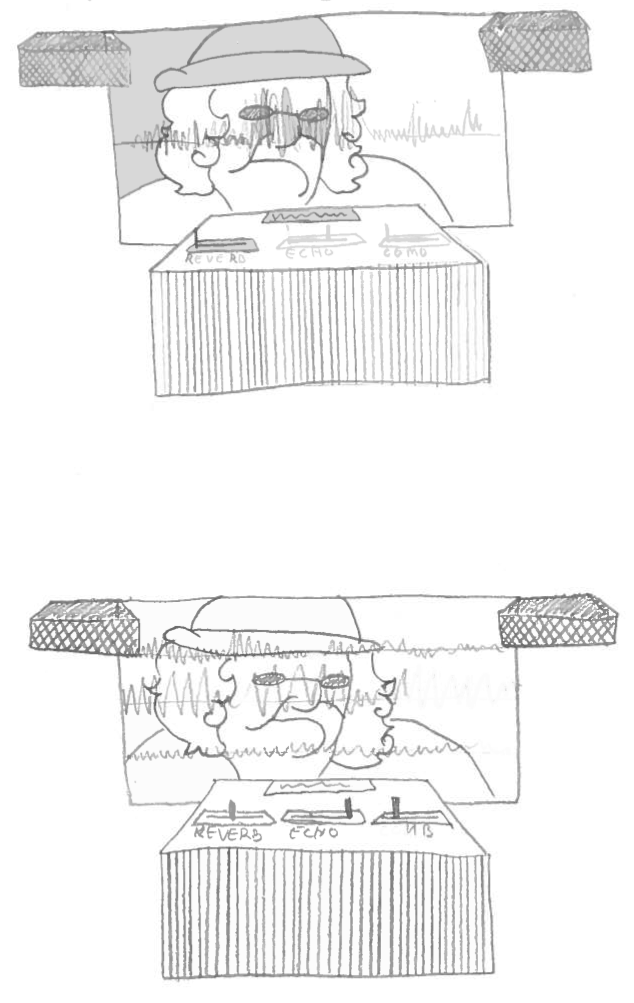
\includegraphics[width=0.5\textwidth]{Visualiseringaflyd}
\caption{\label{fig:Visualiseringaflyd} Sketch on how the sound could be visualised on the image.}
\end{figure}





There are many forms of creative expression including, but not limited to, audio and images, which can be created using various tools. An interesting approach could be to provide artists a new tool of expressing themselves through the use of a physical interface of a device which can transform a digital image into audio. This project aims to explore the creation of audio from images as a tool for such creative expression.



